\section{Methods}
\label{sec:methods}

This section details the computational methodologies employed to learn and utilize nonlinear deformation modes, addressing the challenges of simulating complex soft tissue behavior. We begin by laying the groundwork with a review of fundamental neural network concepts, which are central to our data-driven learning strategy. Following this, we explore the principles of subspace learning, demonstrating how neural networks can be trained to efficiently represent solutions to constrained physical problems. The core of our proposed method, the 'Neural Modes' architecture, is then introduced, including its specific design and the physics-informed loss functions crucial for its training. Finally, we describe the integration of these learned modes into dynamic simulations and discuss potential avenues for extending the framework's capabilities.



\subsection{Neural Network Principles}

A Neural Network (NN) is a mathematical model that achieves statistical generalization drawing inspiration from the human brain. Indeed, it is based on neurons, which are connected one to another, and carry the information from the input to the output.

It is possible to define NN as a function that maps an input to an output, given a set of parameters \( \bm{\theta} \). The function \( \hat{y} = f(\bm{x}; \bm{\theta}) \) is obtained by composing a series of functions \( f_i \) called layers, where each layer is defined as
\begin{equation}
    f_i = \sigma(W_i f_{i-1} + b_i),
\end{equation}
where \( W_i \) is the weight matrix, \( b_i \) is the bias vector and \( \sigma(\cdot) \) is the activation function. The activation function is a non-linear function that allows the network to learn complex patterns in the data. 

A neural network is trained using a dataset \( \mathcal{D} = \{(\bm{x}_i, \bm{y}_i)\}_{i=1}^N \), where \( \bm{x}_i \) is the input and \( \bm{y}_i \) is the corresponding target output. The objective is to find the optimal set of parameters \( \bm{\theta} \) that minimizes a loss function \( \mathcal{L} \), which quantifies the discrepancy between the network's predictions and the true outputs. The loss function is defined as:
\begin{equation}
    \mathcal{L}(\bm{\theta}) = \frac{1}{N} \sum_{i=1}^N L(f(\bm{x}_i; \bm{\theta}), \bm{y}_i)
\end{equation}
where \( L \) is a per-sample loss function (e.g., Mean Squared Error). The optimization process aims to find the parameters \( \bm{\theta}^* \) that minimize the overall loss:
\begin{equation}
    \bm{\theta}^* = \argmin_{\bm{\theta}} \mathcal{L}(\bm{\theta}).
\end{equation}
Common optimization algorithms include Gradient Descent, Adam, and L-BFGS \cite{Liu_1989}.

The full algorithm is the following one:
\begin{algorithm} 
    \caption{Training of a neural network}
    \begin{algorithmic}
        \State Initialize the parameters \( \bm{\theta} \)
        \While{epoch < max\_epochs}
            \For{mini-batch in dataset}
                \State Perform forward pass computing \( f(\bm{x}; \bm{\theta}) \)
                \State Compute the loss function \( \mathcal{L}(f(\bm{x}; \bm{\theta}), \bm{y}) \)
                \State Perform backward pass computing the gradients of the loss function
                \State Update the parameters using the gradients
            \EndFor
        \EndWhile
    \end{algorithmic}
\end{algorithm}



\subsection{Neural Network Architectures}
In this work, we employ a deep residual neural network specifically designed for learning nonlinear deformation modes. This architecture builds upon traditional fully connected neural networks but incorporates residual connections to facilitate the training of deeper networks and improve performance in capturing nonlinear corrections to linear modal displacements.


\subsubsection{Neural Modes Architecture}
The Neural Modes architecture is designed to learn nonlinear corrections to linear deformation modes for Neo-Hookean materials. It consists of a deep residual neural network. The architecture is defined as follows:

\begin{itemize}
    \item The input is a modal coordinate vector \( \bm{z} \in \mathbb{R}^m \), where $m$ is the number of modal coordinates. These modal coordinates represent the weights of the linear modes used to approximate the deformation.
    \item The network consists of several residual blocks, each containing two fully connected layers with Leaky ReLU activation functions, and a skip connection that adds the input of the block to its output. The number of residual blocks and the number of neurons per layer are hyperparameters that can be tuned to optimize performance.
    \item The output layer has a linear activation function and outputs a nonlinear correction to the displacement field \( \bm{y} \in \mathbb{R}^n \), where $n$ is the total number of degrees of freedom in the mesh. This correction is added to the linear modal displacement to obtain a more accurate approximation of the deformed configuration.
\end{itemize}

The network learns to map from the reduced modal space to full-dimensional correction vectors that improve the accuracy of the linear modal approximation. This architecture, which we call Neural Modes, can be visualized as a mapping from a low-dimensional modal space to a high-dimensional displacement space, where the neural network learns to correct the linear approximation provided by the modal basis. The following figure illustrates the architecture:
% H per bloccare la figura. altrimenti metti la referenza
\begin{figure}[H] 
    \centering
    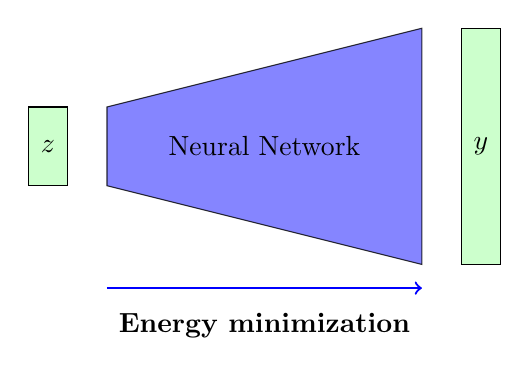
\begin{tikzpicture}
        % Modal coordinate (z)
        \draw[fill=green!20] (-3, 1) rectangle (-2.5,2);
        \node at (-2.75, 1.5) {$\bm{z}$}; % Label inside the rectangle
        
        % Displacement (u)
        \draw[fill=green!20] (2.5,0) rectangle (3,3);
        \node at (2.75, 1.5) {$\bm{y}$}; % Label inside the rectangle
        
        % Energy loss transition
        \draw[fill=blue!60,opacity=0.8] (-2,1) -- (2,-0) -- (2,3) -- (-2,2) -- cycle;
        \node at (0,1.5) {Neural Network};
        \node[below] at (0,-0.5) {\textbf{Energy minimization}};
        
        % Energy loss arrow
        \draw[thick,blue,->] (-2,-0.3) -- (2,-0.3);
    
    \end{tikzpicture}
    \caption{Neural Modes architecture for learning nonlinear deformation corrections}
    \label{fig:neural_modes_arch}
\end{figure}



\subsubsection{Training the Neural Modes}
The training process for the Neural Modes Network is based on minimizing a combination of physics-based losses, rather than simply minimizing the prediction error against ground truth data, which is the classical loss used in most neural network training. The key terms that build the loss used in training are:

\begin{enumerate}
    \item \textbf{Energy Loss}: minimizes the internal strain energy of the deformed configuration $E(\bm{X} + \bm{l} + \bm{y})$, where $\bm{X}$ is the rest position, $\bm{l}$ is the linear mode displacement given by $\bm{z}$, and $\bm{y}$ is the nonlinear correction.
    
    \item \textbf{Orthogonality Loss}: ensures that the nonlinear correction is orthogonal to the linear mode space: $\bm{y}^T \bm{l} = 0$.

    \item \textbf{Boundary Condition Penalty}: enforces the displacement boundary conditions on the deformed configuration.
    
\end{enumerate}

The total loss function is a weighted sum of these individual losses:
\begin{equation}
    \text{Loss} = \text{Energy Loss} + \lambda_1 \text{Orthogonality Loss} + \lambda_2 \text{Boundary Condition Penalty},
\end{equation}
where $\lambda_1$ and $\lambda_2$ are weight parameters that balance the importance of each loss term.

During the training process, we observed that the network tended to learn a non-zero correction even when the input modal coordinate vector was zero (\(\bm{z} = \bm{0}\)), corresponding to the rest position. Ideally, the network's output should be zero at the rest position, indicating no deformation correction. Unlike \cite{Wang_Du_Coros_Thomaszewski_2024}, who address this issue by adding an explicit origin loss term to their loss function, we enforce a zero correction at the origin by using a bias-free neural network architecture. This design choice ensures that the network's output is naturally centered around zero, promoting a zero correction when no modal displacement is applied.

During training, the Neural Modes network is optimized using a self-supervised learning approach, where the loss function is designed to minimize the internal energy of the deformed configuration while enforcing orthogonality and boundary condition constraints. Specifically, we employ the Adam optimizer to minimize a loss function that combines the energy loss with penalty terms for deviations from orthogonality and boundary conditions. The per-sample loss function \( L \) includes a Mean Squared Error (MSE) term for each constraint, ensuring that deviations are quadratically penalized. This approach allows the network to learn the underlying physics of the deformation without relying on precomputed ground truth data.


\subsection{Subspace Learning}
\begin{align}
    \label{eq:constrained_energy_minimization}
    \bm{x}^*(\phi, \psi) = \underset{\bm{x}}{\argmin} \quad & E_\phi(\bm{x}) \\
    \text{s.t.} \quad & C_\psi(\bm{x}) = 0, \nonumber
\end{align}
where \( E_\phi \) is the energy function defined by parameters \(\phi\) and \( C_\psi \) is the constraint function with parameters \(\psi\). The solution set \( \bm{x}^*\) constitutes a subspace of the full-dimensional space \( \mathbb{R}^d \). In a classical Finite Element framework, sampling from this subspace is achieved by solving a constrained minimization problem for each configuration. 

Clearly, this approach is computationally expensive, so we need a more efficient way to sample from the subspace.

The idea proposed by \cite{Wang_Du_Coros_Thomaszewski_2024} is to find a Neural Network \( \bm{x}[\theta^*](\phi, \psi) \) that approximates the solution \( \bm{x}^* \), meaning that the problem becomes:
\begin{align*}
    \bm{x}[\theta^*](\phi, \psi) \approx \underset{\theta}{\argmin} \quad & E_\phi(\bm{x}[\theta](\phi, \psi)) \\
    \text{s.t.} \quad & C_\psi(\bm{x}[\theta](\phi, \psi)) = 0.
\end{align*}

Now, defining the nonlinear modes as 
\begin{align}
    \bm{n}(\bm{z}) = \bm{l} + \argmin_{\bm{y}} \quad & E_\phi(\bm{X} + \bm{l} + \bm{y}) \\ 
    \text{s.t.} \quad & \bm{l}^T \bm{y} = 0,
\end{align}
where \( \bm{l} \) is the linear mode displacement obtained as
\begin{equation}
    \bm{l} = \sum_{i=1}^m z_i \bm{e}_i,
\end{equation}
where \( \bm{e}_i \) is the $i$-th linear mode and \( z_i \) is the corresponding modal coordinate, we can rewrite the problem \ref{eq:constrained_energy_minimization} as:
\begin{align*}
    \bm{n}[\theta^*](\bm{z}) &= \bm{l} + \bm{y}[\theta^*](\bm{z}), \\
    \theta^* = \underset{\theta}{\argmin} \quad & E_\phi(\bm{X} + \bm{l} + \bm{y}[\theta](\bm{z})) \\
    \text{s.t.} \quad & \bm{l}^T \bm{y}[\theta](\bm{z}) = 0.
\end{align*}

Now we define a suitable function that will serve as a loss function for the self-supervised training of the neural network. The loss function is defined as:
\begin{equation}
    \mathcal{L}(\theta) = \mathbb{E}_{\bm{z}} \left[ E(\bm{X} + \bm{l} + \bm{y}[\theta](\bm{z})) + \lambda_1 \bm{l}^T \bm{y}[\theta](\bm{z}) + \lambda_2 \text{B. C. Penalty} \right],
\end{equation}
where \( \lambda_1 \) and \( \lambda_2 \) are hyperparameters that control the importance of the orthogonality and boundary condition penalty terms, respectively. The first term is the energy loss, which minimizes the internal strain energy of the deformed configuration, while the second term ensures that the nonlinear correction is orthogonal to the linear mode space. The third term enforces the displacement boundary conditions on the deformed configuration.

\subsection{Sampling the Modal Space}
One of the main challenges for this method is finding a good way to sample the \(z\) vector that will be used as input for the neural network. Here are two examples that shows how choosing randomly the \(z\) vector can lead to unrealistic results. 
\begin{figure}[H]
    \centering
    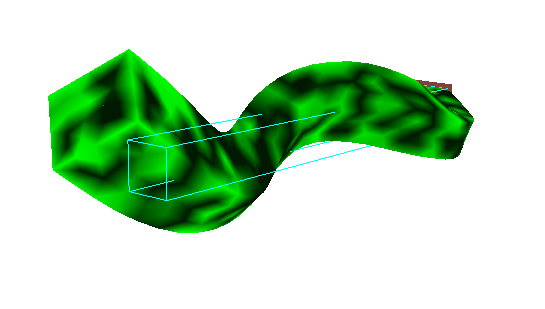
\includegraphics[width=0.4\textwidth]{Images/z_random.png}
    \caption{Example of a bad sampling of the modal space, the reference shape is the light blue outline.}
    \label{fig:bad_sampling}
\end{figure}
In this example, the random \(z\) vector has large values in its latter components. These components represent higher-frequency deformation modes, which naturally contain more strain energy. Using these modes with high amplitudes often creates physically unrealistic or extreme configurations. This shows why random sampling across all components of \(z\) can lead to unrealistic deformations.

A better sampling approach considers the physical meaning of each mode. The first components of \(z\) typically correspond to lower-frequency, global deformation modes that represent major shape changes with less energy. Later components represent higher-frequency, localized, and more energetic modes. 

For more effective sampling of the modal space, we can implement a strategic approach to generating the \(z\) vectors. This approach involves assigning larger coefficient values to the first several components of the vector, which typically correspond to the fundamental, lower-frequency deformation modes, while progressively reducing the magnitude of values assigned to later components. By structuring our sampling in this manner, the resulting deformations tend to be significantly more physically realistic and energetically feasible in real-world scenarios. This methodical sampling focuses the neural network's training process on common, naturally occurring deformation patterns rather than directing computational resources toward unlikely, high-energy configurations that rarely manifest in practical applications.

The fundamental issue with purely random sampling across all modal coordinates is that it inadvertently forces the neural network to attempt energy minimization for physically implausible states. Given that the energy landscape for soft tissue deformation is already inherently complex and high-dimensional, introducing this additional unnecessary complexity substantially increases the difficulty of the training process and potentially compromises the quality of the learned model. This consideration underscores the necessity for developing a more sophisticated and physically-informed strategy to efficiently sample the modal space, allowing the network to concentrate on learning the most relevant aspects of the deformation behavior.


\subsection{Dynamic Simulation with Neural Modes}
For dynamic simulations, the Neural Modes framework solves an optimization problem at each time step. Given the current and previous displacement states $\bm{u}_n$ and $\bm{u}_{n-1}$, the modal coordinates for the next time step $\bm{z}_{n+1}$ are computed by:
\begin{equation}
    \bm{z}_{n+1} = \underset{\bm{z}}{\argmin} \frac{1}{2h^2} \|\bm{n}(\bm{z}) - 2\bm{u}_n + \bm{u}_{n-1}\|_{\bm{M}}^2 + E(\bm{n}(\bm{z})),
\end{equation}
where $\bm{n}(\bm{z})$ represents the complete displacement field (linear modes plus nonlinear correction), $h$ is the time step, $\bm{M}$ is the mass matrix, and $E(\cdot)$ is the internal energy of the configuration. This optimization problem is typically solved using the L-BFGS-B algorithm \cite{Liu_1989}.

One challenge with this approach is that the optimization problem does not explicitly account for external forces. The network learns to minimize internal energy but lacks direct information about external forces that may be applied during simulation: this limitation can affect the accuracy of dynamic simulations, particularly for large deformations or complex loading conditions.



